%!TEX root = thesis.tex
\section{Small Boat Fleet and Shipping Decarbonisation}
Current literature related to estimating small-scale vessels without machine learning methods includes using statistical factors or measures.~\newcite{johnson2017spatial} used Kernel Density Estimation (KDE) to distribute data on the population, the number of ships, and the average annual total catch for the entire population, and finally showed that their forecasts could accurately predict the landing of fisheries in the bay. In their paper, they explained the source of their data~\cite{Lopez-Sagastegui2017Comparing}. Lopez-Sagastegui et al. worked with fishers to generate and record information about fish catches, fishing efforts, profits, species breeding seasons, and spatial patterns of fishing activities. However, one of the points against this work is that it only focuses on fishing vessels. While these are the majority, it still misses the other ship types. Notably, the authors provided information (Figure~\ref{review_density_of_gulf}) of the density of human population and boats in the Gulf of California that can save much time in creating data sets of the Gulf of California for training machines learning models.

\begin{figure}[!t]
\center
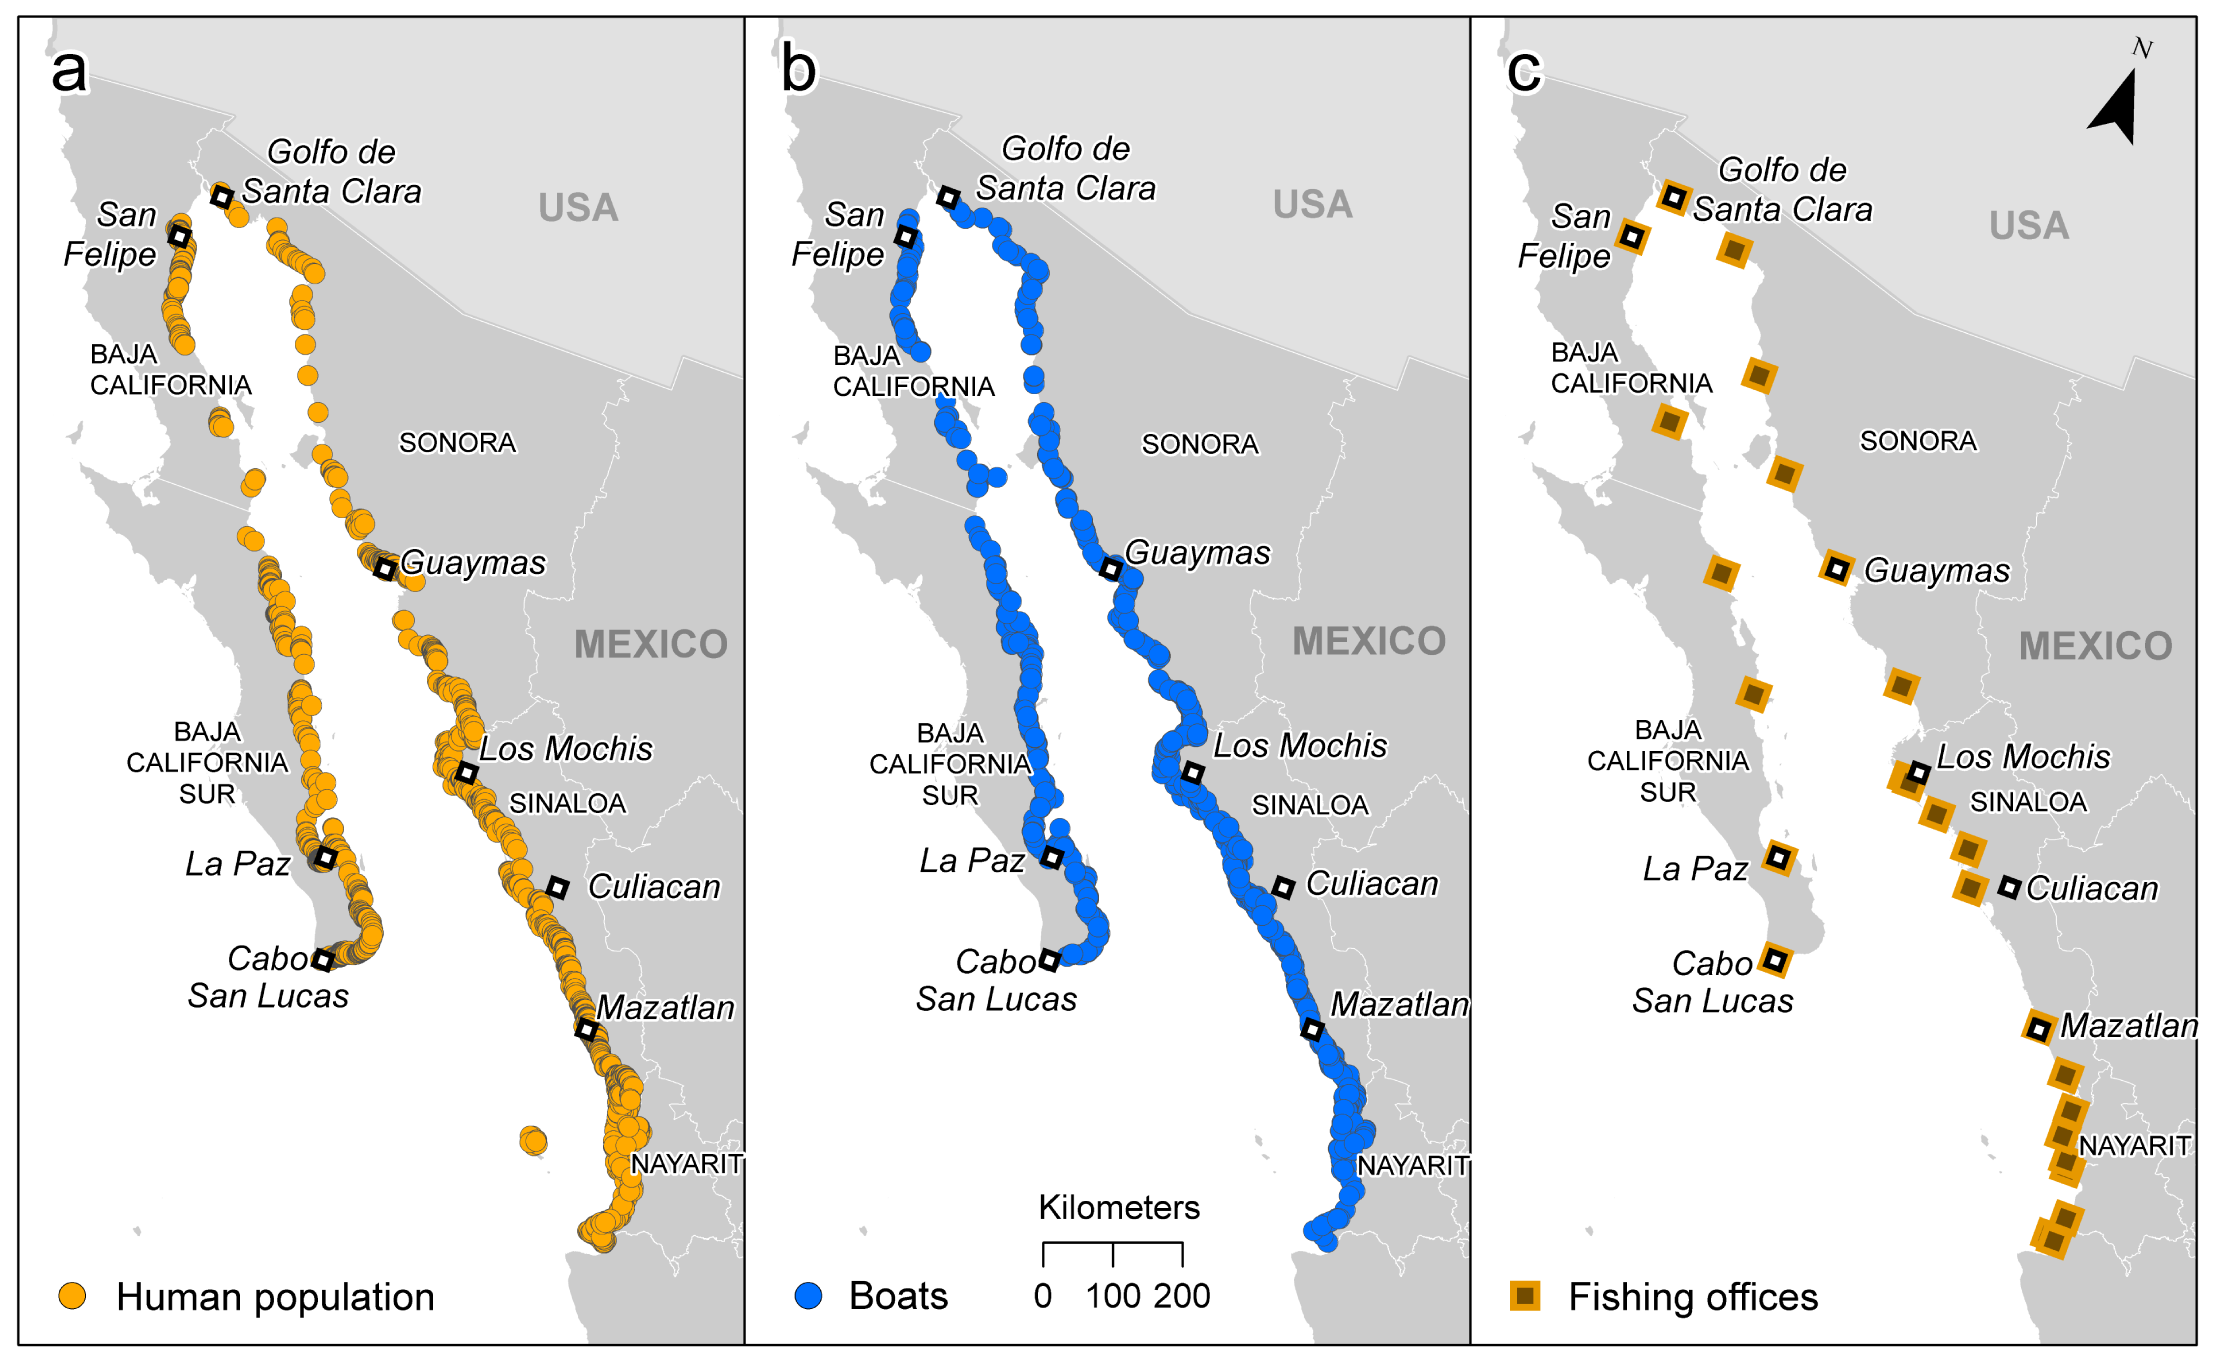
\includegraphics[scale=0.7]{img/review_density_of_gulf.png}
\longcaption{Map of the density of human population, boats, and fishing offices in the Gulf of California.}{\label{review_density_of_gulf} Map of the density of human population, boats, and fishing offices in the Gulf of California~\cite{johnson12exequiel}.}
\end{figure}

~\newcite{Johansson2018ModelingOL} proposed a new model (FMI-BEAM) to describe the emissions of the leisure boat fleet in the Baltic Sea region with over 3000 dock locations, national small boat registry, AIS data and vessel survey results. However, the method cannot cover countries with no national registry for small boats. Besides, small boats are not just leisure boats.~\newcite{Ug2020EstimationOW} estimated global ship emissions with the help of data from the Automatic Identification System (AIS). They set up movement information relating to ship size and speed and meteorological and marine environmental conditions. Over 3,000,000,000 daily AIS data records from hundreds of owners and thousands of partner AIS base stations and detailed ship data. However, this method is highly dependent on AIS data which is impossible for unregistered small boats.~\newcite{Traut2013MonitoringSE, Johansson2016ACM, Mabunda2014EstimatingCD, Hensel2020GreenSU, Han2016RealtimeIA} have proposed the use of AIS to monitor the carbon emissions of the fleet as well.

~\newcite{Zhang2019TheSO} included unidentified vessels in the AIS-based vessel emission inventory. They developed an AIS-instrumented emissions inventory, including both identified and unidentified vessels. In particular, missing vessel parameters for unidentified vessels were estimated from a classification regression of vessels with similar vessel types and sizes in the AIS database. However, the authors do not discuss whether the regression model applies to vessels in most coastal areas of the planet. In addition, the authors do not discuss whether the vessel data in the AIS database is regionally diverse. Finally, if there is a diversity of vessels in the AIS database, the authors did not discuss whether this diversity would produce more significant errors in the predictions for small vessels in a single region (e.g. the Gulf of California, Mexico).




\newpage
\section{Convolutional Neural Networks in Image Recognition}
\label{sec2.2}
Literature tends to be inaccurate for emission inventories for the small boat fleet. The above literature review has demonstrated that there is still a lot of work to understand how the small boat fleet is being operated, what fuels they are using, and the level of activity for this shipping sector. This master thesis project intends to use image recognition algorithms to detect small boats in any sea area, significantly reducing the time to calculate small vessel emission inventories. Besides, it will be in the national interest for the small fleet to account for and control these emissions within the powers of the state, incentivising the energy-efficient technologies and fuel change. Further, if countries meet their ambitious net-zero carbon emissions targets, they cannot afford to ignore the small boat fleet emission inventories that can help governments account for carbon emissions from small boats more quickly.

The goal of target detection, which is to determine the location of a target in an image based on a large number of predefined classes, is one of the most fundamental and challenging problems in computer vision. Deep learning techniques, which have emerged in recent years, are a powerful method for learning features directly from data and have led to significant breakthroughs in the field of target detection. Furthermore, with the rise of self-driving cars and face detection, the need for fast and accurate object detection is growing.

In 2012, AlexNet, a deep convolutional neural network (DCNN) proposed by ~\newcite{krizhevsky2012imagenet}, achieved record accuracy in image classification at the ImageNet Large-Scale Visual Recognition Challenge (ILSRVC), making convolutional neural networks the dominant paradigm for image recognition. Then, ~\newcite{girshick2014rich} introduces Region-Based Convolutional Neural Networks (R-CNN), the first convolutional neural network (CNN)-based object detection method. The R-CNN algorithm represents a two-step approach, where a region proposal is generated firstly, and then a CNN is used for recognition and classification. Compared to the traditional sliding convolutional window to determine the possible regions of objects, R-CNN uses selective search to pre-extract some candidate regions that are more likely to object to avoid computationally costly classification and object search, which is much faster and significantly less expensive~\cite{ uijlings2013selective, girshick2014rich}. Overall, the R-CNN approach is divided into four steps.

\begin{itemize}
    \item Generating candidate regions;
    \item Feature extraction using CNN on the candidate regions;
    \item Feeding the extracted features into a support vector machine (SVM) classifier;
    \item Finally, the object positions are corrected using a regressor;
\end{itemize}

However, R-CNN also has many drawbacks: the selective search method is very slow in generating positive and negative sample candidate regions for the training network, which affects the overall speed of the algorithm; the CNN needs to perform feature extraction once for each generated candidate region separately, and there are a large number of repeated operations, which limits the algorithm performance ~\cite{huang2017speed}.


Since its inception, R-CNN has undergone several developments and iterations: Fast R-CNN, Faster R-CNN and Mask R-CNN~\cite{girshick2015fast, ren2015faster, he2017mask}. The improvement of Fast R-CNN is the design of a pooling layer structure for ROI (Region of Interest) Pooling, which effectively solves the operation of R-CNN algorithms that must crop and scale image regions to the same size. Faster R-CNN replaces the selective search method with RPN (Region Proposal Network) ~\cite{ren2015faster}. The selection and judgment of candidate frames are handed over to the RPN for processing, and the candidate regions after RPN processing are subjected to multi-task loss-based classification and localization. 

Several convolutional neural network-based object detection frameworks have recently emerged that can run faster, have a higher detection accuracy, have cleaner results and are easier to develop. Compared to the Faster RCNN model, the YOLO model can better detect smaller objects, for example, by easily detecting smaller traffic lights at a distance (Dwivedi, 2020) (Figure 3.7, Figure 3.8), which is important when detecting satellite images. Also, the YOLO model has a faster end-to-end runtime and detection accuracy than the Faster RCNN. For example, the figures below is from a YouTube clip of an NBA game. As seen in Figure 3.9 and Figure 3.10, the detection accuracy under the YOLO model is more accurate than that of the Faster RCNN. This helps to monitor the number of small boats in real-time using the YOLO model in the future.


\begin{figure}[p]
    \centering
    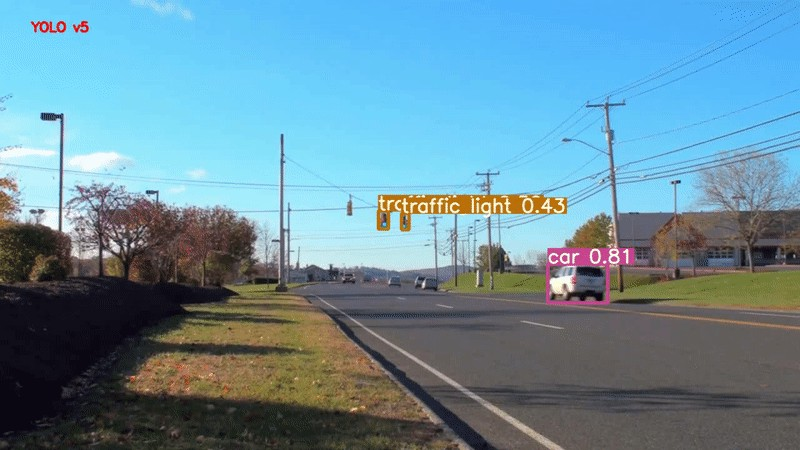
\includegraphics[scale=0.5]{img/who_wins_traffic_light_YOLO.jpg}
    \longcaption{YOLOv5 model in a driving video.}{YOLOv5 model in a driving video~\cite{Dwivedi2020YOLOv5}.}
    \label{fig:who_wins_traffic_light_YOLO}
\end{figure}

\begin{figure}[p]
    \centering
    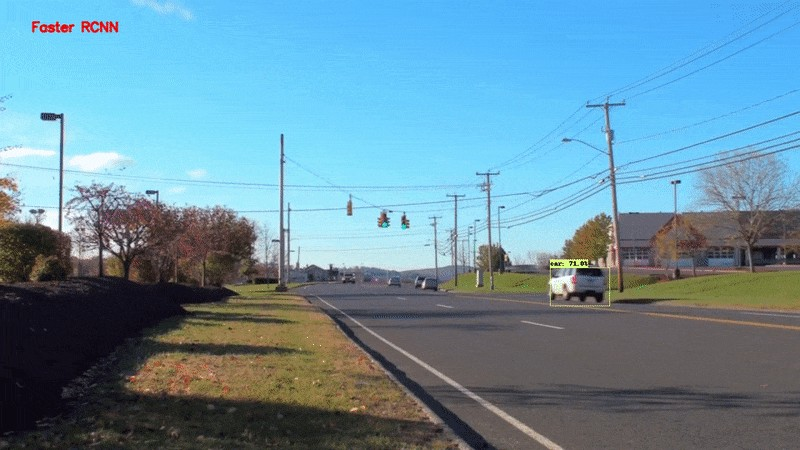
\includegraphics[scale=0.5]{img/who_wins_traffic_light_RCNN.jpg}
    \longcaption{Faster RCNN model in a driving video.}{Faster RCNN model in a driving video~\cite{Dwivedi2020YOLOv5}.}
    \label{fig:who_wins_traffic_light_RCNN}
\end{figure}

\begin{figure}[p]
    \centering
    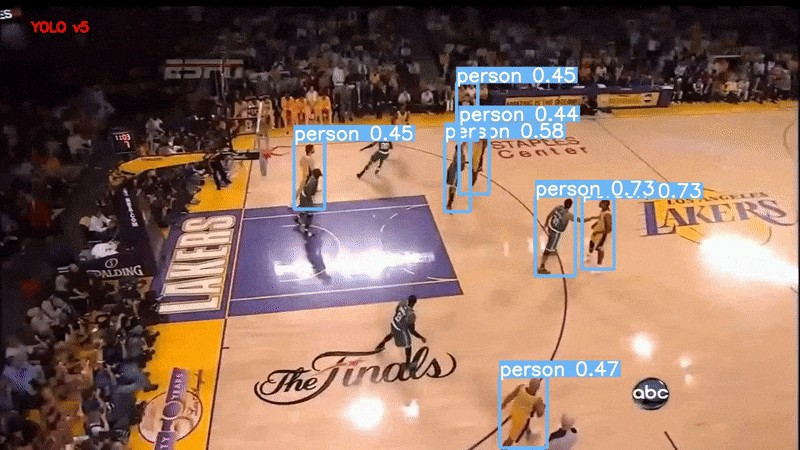
\includegraphics[scale=0.5]{img/who_wins_nba_YOLO.jpg}
    \longcaption{YOLOv5 model in an NBA game video.}{YOLOv5 model in an NBA game video~\cite{Dwivedi2020YOLOv5}.}
    \label{fig:who_wins_nba_YOLO}
\end{figure}

\begin{figure}[p]
    \centering
    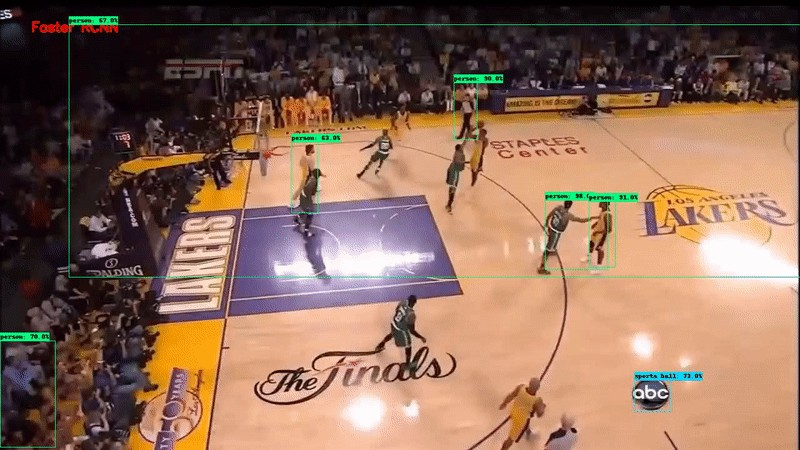
\includegraphics[scale=0.5]{img/who_wins_nba_RCNN.jpg}
    \longcaption{Faster RCNN model in an NBA game video.}{Faster RCNN model in an NBA game video~\cite{Dwivedi2020YOLOv5}.}
    \label{fig:who_wins_nba_RCNN}
\end{figure}

Mask R-CNN upgrades the ROI Pooling layer of Fast R-CNN to an ROI Align layer and adds a branching FCN layer, the mask layer, to the bounding box recognition for semantic mask recognition ~\cite{he2017mask}. Thus, the Mask R-CNN is essentially an Instance Segmentation algorithm, compared to Semantic Segmentation. Instance Segmentation is a more fine-grained segmentation of similar objects than Semantic Segmentation.

However, even traditional CNNs can be very useful for large-scale image recognition.~\newcite{Simonyan2015VeryDC} from the University of Oxford and Google DeepMind researched the effect of convolutional network depth on its accuracy in the large-scale image recognition setting. Their research found out that even they used very small (3x3) convolution filters, a significant improvement can be achieved by pushing the depth to 16 to 19 weight layers.


\section{Noise Removal for Image in the Shipping Sectors or Similar Applications}
Satellite images often have noises that should not be there, such as shadows cast by water on the sea surface due to sunlight or clouds in the atmosphere. These noises can make the training data inaccurate and often cause problems for the correctness of the model.~\newcite{He2009SingleIH} proposed a simple but effective image prior-dark channel before removing haze from a single input image. The dark channel prior is a kind of statistics of outdoor haze-free images. Based on critical observation, most local patches in outdoor haze-free images contain some pixels whose intensity is very low in at least one colour channel. Using this before the haze imaging model, the thickness of the haze can be estimated, and a high-quality haze-free image can be recovered. Moreover, a high-quality depth map can also be obtained as a byproduct of haze removal.\\

In summary, past literature on carbon inventories of shipping has not focused on small vessels. However, with the development and maturation of a range of computer vision techniques such as convolutional neural networks, it may be possible to identify small vessels from open satellite imagery accurately. In the next section, I will first explain how object detection models can be trained through a convolutional neural network-based YOLO architecture.